%!TEX root = ../main.tex

\section{Preliminaries}\label{sec:preliminaries}
We employ standard terminology from (finite and classical) model theory~\cite[Sec. 1--3]{Libkin04}.
A quick reference of all notation used in this paper is given in \cref{fig:notation-quickref}.

\begin{figure}
  \centering
  \bgroup
  \def\arraystretch{1.1}
  \begin{tabularx}{\textwidth}{c X r}
    notation & meaning & introduced in \\
    \hline
    $\str{A}$, $\str{B}$, \ldots & structures with domains $A$, $B$, \ldots & \cref{sec:preliminaries} \\
    $\Sigma$ & the signature of all structures in this paper (purely relational) & \cref{sec:preliminaries} \\
    $\arity(\Sigma)$ & the maximum arity among all predicates in $\Sigma$ (width of $\Sigma$) & \cref{sec:preliminaries} \\
    $\elemtuplea, \elemtupleb$, \ldots & tuples of elements & \cref{sec:preliminaries} \\
    $\elemtuptuplea, \elemtuptupleb$, \ldots & tuples of tuples / tuples of elements from unravelings & \cref{sec:preliminaries} \\
    $f[\elemtuplea]$ & componentwise-image of $f$ on $\elemtuplea$, i.e.\ $(f(a_{1}), \ldots, f(a_{n}))$ & \cref{sec:preliminaries} \\
    $\tp{\logicL}{\str{A}}{\elemtuplea}$ & $\logicL[\sigma]$-type of $\elemtuplea$ in $\str{A}$ (all $\logicL[\sigma]$-formulaes satisfied by $\elemtuplea$) & \cref{sec:preliminaries} \\
    $\atp{\logicL}{\str{A}}{\elemtuplea}$ & atomic-$\logicL[\sigma]$-type of $\elemtuplea$ in $\str{A}$ & \cref{sec:preliminaries} \\
    $\logicL_{\ell}$ & logic $\logicL$ restricted to formulae with quantifier rank at most $\ell$ & \cref{sec:preliminaries} \\
    $\str{A}, \elemtuplea \bisimto_{\FGF} \str{B}, \elemtupleb$ & an $\FGF$-bisimulation containing $(\elemtuplea, \elemtupleb)$ exists between $\str{A}$ and $\str{B}$ & \cref{sec:preliminaries} \\
    $\str{A}, \elemtuplea \bisimto_{\FGF}^{\ell} \str{B}, \elemtupleb$ & an $\ell$-$\FGF$-bisimulation containing $(\elemtuplea, \elemtupleb)$ exists between $\str{A}$ and $\str{B}$ & \cref{sec:preliminaries} \\
    $\unravel{A}$ & the (possibly infinite) tree unraveling of $\str{A}$ & \cref{sec:unraveling} \\
    $\unravel{A}_{\ell}$ & the finite unraveling of $\str{A}$ for threshold $\ell$ & \cref{sec:finite} \\
    $\relNext$ & the parent-child relation in the tree unraveling & \cref{sec:unraveling} \\
    $\relNext_{\ell}$ & finitary variant of $\relNext$, used for defining $\unravel{A}_{\ell}$ & \cref{sec:finite} \\
    $\seq{a}$ & sequence part of an unraveling element, i.e.\ $\sigma$ for $a = (\sigma, k)$ & \cref{sec:unraveling} \\
    $\ctr{a}$ & counter part of an unraveling element, i.e.\ $k$ for $a = (\sigma, k)$ & \cref{sec:unraveling} \\
    $\bound{\elemtuptuplea}$ & counter of the last component of $\elemtuptuplea$, i.e.\ $\ctr{a_{|\elemtuptuplea|}}$ & \cref{sec:unraveling} \\
  \end{tabularx}
  \egroup
  \caption{Overview of relevant notation. Some of these are only introduced later in this paper.}\label{fig:notation-quickref}
\end{figure}

All the logics considered in this paper are fragments of the first-order logic ($\FO$) over purely-relational equality-free vocabularies, under the usual syntax and semantics. 
We fix a countably infinite set $\V \deff \{x_i \colon\, i \in \N\}$ of variables and a countably infinite set~$\R$ of predicates (we employ $\arity(\relR)$ to denote the arity of $\relR$ from $\R$).
Throughout this paper all formulae use variables from $\V$ and predicates from a fixed, finite signature $\Sigma$ which is a subset of $\R$.
Since $\Sigma$ is finite, there is a maximum arity of any relation in $\Sigma$, which we denote by $\arity(\Sigma)$.
Given a formula $\varphi$ we use $\sig(\varphi)$ to denote the set of predicates appearing in $\varphi$. 
We write $\varphi(\vartuplex)$ to indicate that all free variables from $\varphi$ are members of $\vartuplex$. 
If $\vartuplex$ contains precisely the free
variables of $\varphi$, then we emphasise this fact separately.
A formula without free variables is called a \emph{sentence}.
Given a structure $\str{A}$ and $B \subseteq A$, we use $\restr{\str{A}}{B}$ to denote the \emph{substructure} of $\str{A}$ induced by $B$.\\

\noindent \textbf{Tuples and subsequences.}
An $n$-tuple is a list of $n$ elements.
Given a tuple $\elemtuplea$ we use $\set(\elemtuplea)$ to denote the set of its components. 
The $0$-tuple is denoted with~$\emptytupl$.
We use $\vartuplexfromto{i}{j}$ to denote the $(j{-}i{+}1)$-tuple $\varx_i, \varx_{i+1}, \ldots, \varx_j$.
We say that $\vartuplexfromto{i}{j}$ is an infix of a tuple $\vartuplexfromto{k}{l}$ if $k \leq i \leq j \leq l$ holds.
We use the notation ``$\cdots e$'' for a tuple where the last element is equal to $e$ and preceding elements are not important.
For a function $f$ and tuple $\elemtuplea_{1\ldots\ell}$, we write $f[\elemtuplea_{1\ldots\ell}]$ for the tuple $(f(a_{1}), \ldots, f(a_{\ell}))$.
To improve readability, tuples of tuples are denoted by arrows, for instance with $\elemtuptuplea$.
For a set $S$, we write $\vartuplex \sqin S$ iff $\varx_i \in S$ for all indices $1 \leq i \leq |\vartuplex|$, where $|\vartuplex|$ denotes the length of~$\vartuplex$. 
We say that a tuple $\elemtuplea \sqin A$ is \emph{live} in $\str{A}$ if $|\elemtuplea| \leq 1$ or~$\elemtuplea \in \relR^{\str{A}}$ for some predicate~$\relR \in \Sigma$.\\

\noindent \textbf{Types and logical equivalence.}
Fix a logic $\logicL$ and a finite signature~$\sigma \subseteq \R$. 
We~employ~$\logicL[\sigma]$ in place of~$\{ \varphi \in \logicL \colon\,  \sig(\varphi) \subseteq \sigma \}$.
Since all structures and formulae throughout this paper use a fixed signature $\Sigma$, we omit the signature from now on and write just $\logicL$ instead of $\logicL[\Sigma]$.
Moreover, we use $\logicL_\ell$ to denote the restriction of $\logicL$ to formulae of \emph{quantifier rank} (i.e.\ the maximal number of nested quantifiers) at most~$\ell$.
%
The \emph{$\logicL$-type} of $\elemtuplea$ in $\str{A}$, denoted with~$\tp{\logicL}{\str{A}}{\elemtuplea}$, consists of all $\logicL$-formulae with free variables~$\vartuplexfromto{1}{n}$ that are satisfied by $\elemtuplea$ in $\str{A}$.
If we restrict the type to only atomic and negated atomic $\logicL$-formulae, we obtain the \emph{atomic-$\logicL$-type} of $\elemtuplea$ in $\str{A}$, denoted with~$\atp{\logicL}{\str{A}}{\elemtuplea}$.
The atomic-$\logicL$-type of $\elemtuplea$ is logically equivalent to the $\logicL_{0}$-type of $\elemtuplea$ in $\str{A}$.
We write $\str{A} \equiv_\logicL \str{B}$ if $\str{A}$ and~$\str{B}$ satisfy the same $\logicL$-sentences.
For pointed structures $(\str{A}, \elemtuplea), (\str{B}, \elemtupleb)$ with $n$-tuples $\elemtuplea$ and~$\elemtupleb$ we employ the notation $(\str{A}, \elemtuplea) \equiv_\logicL (\str{B}, \elemtupleb)$ to indicate that for all $\varphi \in \logicL$ with free variables contained in the set $\{ \varx_1, \ldots, \varx_n \}$ we have $\str{A} \models \varphi[\elemtuplea]$ if and only if $\str{B} \models \varphi[\elemtupleb]$ (here variables $\varx_i$ are substituted, respectively, for $\elema_i$ and $b_i$).\\

\noindent \textbf{Guarded fragments.}
We recall the definition of the \emph{guarded fragment}~\cite[Sec. 4.1]{AndrekaNB98}, \ie the fragment of $\FO$ obtained by requiring that blocks of quantifiers are appropriately relativised by atoms.
Formally $\GF$ is the smallest fragment of $\FO$  such that:
\begin{itemize}\itemsep0em
    \item Every atomic formula is in $\GF$;
    \item $\GF$ is closed under boolean connectives $\land, \lor, \neg, \to$;
    \item If $\varphi(\vartuplex, \vartupley)$ is in $\GF$, $\alpha(\vartuplex, \vartupley)$ is an atom containing all free variables of $\varphi$, and $\vartupley$ is a tuple of variables then both $\forall{\vartupley} \; (\alpha(\vartuplex, \vartupley) \to \varphi(\vartuplex, \vartupley))$ and $\exists{\vartupley} \; (\alpha(\vartuplex, \vartupley) \land \varphi(\vartuplex, \vartupley))$ are in $\GF$; 
    \item If $\varphi(\varx)$ has only a single free-variable $\varx$, then $\forall{\varx}\; \varphi(\varx)$ and $\exists{\varx}\; \varphi(\varx)$ are in $\GF$.
\end{itemize}
The predicates $\alpha$ appearing in the 3rd item of the above definition are called \emph{guard} for $\varphi$.
We~stress that in definition of a quantifier rank for $\GF$ we treat quantifiers $\exists{\vartuplex}$ introducing tuples of variables as a single quantifier (not as an abbreviation for a block of quantifiers).

\begin{example}
A formula $\exists{x_{1}x_{2}x_{3}}\; (\relR(x_{1}, x_{2}, x_{3}) \land \forall x_{4}(\relR(x_{4}, x_{4}, x_{1}) \to \relR(x_{1}, x_{4}, x_{1})))$ belongs to $\GF$, but the formula $\exists{x_{1}x_{2}x_{3}}\; (\relE(x_{1}, x_{2}) \land \relE(x_{2}, x_{3}) \land \relE(x_{3}, x_{1}))$ does not.
\end{example}

The \emph{forward guarded fragment}~\cite[Sec. 3.1]{Bednarczyk21} (or $\FGF$) restricts $\GF$ in a way that the allowed sequences of atoms are infixes of the sequence of already-introduced variables (in the order of their quantification).
A formal definition comes next, which will be followed by a bunch of examples.
Let $\FGF(n)$ for $n \in \N$ be the smallest fragment of $\FO$ satisfying:
\begin{itemize}\itemsep0em
    \item An atom $\alpha(\vartuplex)$ belongs to $\FGF(n)$ if $\alpha$ is equality-free and $\vartuplex$ is an infix of $\vartuplexfromto{1}{n}$.
    \item $\FGF(n)$ is closed under boolean connectives $\land, \lor, \neg, \to, \iff$;
    \item If $\alpha$ and $\varphi$ are in $\FGF(n{+}k)$ for a positive $k$ where $\alpha(\vartuplex, \vartupley)$ is an atom containing all free variables of $\varphi$ and $\vartupley$ is a $k$-tuple of variables then $\forall{\vartupley} \; (\alpha(\vartuplex, \vartupley) \to \varphi(\vartuplex, \vartupley))$ and $\exists{\vartupley} \; (\alpha(\vartuplex, \vartupley) \land \varphi(\vartuplex, \vartupley))$ are both in $\FGF(n)$;
    \item If $\varphi(\varx_1) \in \FGF(1)$ has only a single free-variable $\varx_1$, then $\forall{\varx_1}\; \varphi$ and $\exists{\varx_1}\; \varphi$ are in $\FGF(0)$.
\end{itemize}
We use $\FGF$ to denote $\FGF(0)$. Note that $\FGF(0)$ is solely composed of sentences. 

\begin{example}
A formula $\exists{x_1x_{2}x_{3}}\; [\relR(x_{1}, x_{2}, x_{3}) \land \forall{x_{4}x_{5}}(\relS(x_{3}, x_{4}, x_{5}) \to \relT(x_{4})) \land \exists{x_{3}}(\relR(x_{1}, x_{2}, x_{3}))]$ belongs to $\FGF$.
Moreover, first-order translations of (polyadic) modal and description logics are also in $\FGF$.
In contrast, formulae $\exists{x_{1}}\; \relE(x_{1}, x_{1})$ and $\exists{x_{1}}\; (\forall{x_{2}} \relT(x_{1}, x_{2}))$ are not in $\FGF$.
For the former formula the reason is that the sequence $x_1x_1$ is not an infix of the sequence~$x_1$.
The latter formula is not even in $\GF$ as the sequence $x_{1}, x_{2}$ is not guarded.
\end{example}

\noindent \textbf{Bisimulations for guarded fragments.}
%
We next present notion of bisimulation relations tailored towards $\GF$ and $\FGF$, based on presentations from~\cite[Sec. 2.2.3]{Otto04} and~\cite[Sec. 2]{BednarczykJ22}.

For structures $\str{A}$ and $\str{B}$ we denote with $\PartIso{\str{A}}{\str{B}}$ the set of all partial isomorphisms between $\str{A}$ and $\str{B}$.
For non-empty $\bisimY, \bisimZ \subseteq \PartIso{\str{A}}{\str{B}}$ we say that $\bisimZ$ satisfies back-and-forth conditions for $\bisimY$ if for every partial isomorphism $\partisof \in \bisimY$ we have:
%
\begin{description}\itemsep0em
  \item[\desclabel{(Forth)}{bisim:forth}] For every live $\elemtuplea$ in $\str{A}$, there is $\partisog \in \bisimZ$ with the domain $\set(\elemtuplea)$ such that $\partisof$ and $\partisog$ agree on their common domain.
  \item[\desclabel{(Back)}{bisim:back}] For every live $\elemtupleb$ in $\str{B}$, there is $\partisog \in \bisimZ$ with the image $\set(\elemtuplea)$ such that $\partisof$ and $\partisog$ agree on their common image.
\end{description}
A non-empty set $\bisimZ \subseteq \PartIso{\str{A}}{\str{B}}$ is a $\GF$-\emph{bisimulation} between $\str{A}$ and $\str{B}$ if it itself satisfies \ref{bisim:forth} and~\ref{bisim:back} conditions given above.
An $\ell$-$\GF$-bisimulation between $\str{A}$ and $\str{B}$ is a sequence of sets $\bisimZ_0, \bisimZ_1, \ldots, \bisimZ_\ell \subseteq \PartIso{\str{A}}{\str{B}}$ such that for all $i < \ell$ we have that $\bisimZ_i$ satisfies~\ref{bisim:forth} and~\ref{bisim:back} conditions for $\bisimZ_{i{+}1}$.
We say that pointed structures $(\str{A}, \elemtuplea)$ and~$(\str{B}, \elemtupleb)$ are $\GF$-\emph{bisimilar}, denoted $(\str{A}, \elemtuplea) \bisimto_{\GF} (\str{B}, \elemtupleb)$, if there exists a $\GF$-bisimulation between $\str{A}$ and $\str{B}$ containing the partial isomorphism that maps $\elemtuplea$ to $\elemtupleb$.
We analogously speak about $\ell$-$\GF$-\emph{bisimilarity} and employ the notation $(\str{A}, \elemtuplea) \bisimto_{\GF}^{\ell} (\str{B}, \elemtupleb)$.
We use the notation $\elemtuplea \bisimto_{\GF} \elemtupleb$ or $\elemtuplea \bisimto_{\GF}^{\ell} \elemtupleb$ if the structures $\str{A}$ and $\str{B}$ are clear from the context.

The following classical lemma links bisimulations and logical~equivalence.
\begin{lemma}[Thm. 1.12 of~\cite{Gradel014}]\label{lemma:GF-bisimulations-work-well}
For every pair of pointed structures $(\str{A}, \elemtuplea)$ and~$(\str{B}, \elemtupleb)$ we have that:
\begin{enumerate}[(a)]
\item $(\str{A}, \elemtuplea) \bisimto_{\GF} (\str{B}, \elemtupleb)$ implies $(\str{A}, \elemtuplea) \equiv_{\GF} (\str{B}, \elemtupleb)$;
\item $(\str{A}, \elemtuplea) \bisimto_{\GF}^{\ell} (\str{B}, \elemtupleb)$ implies $(\str{A}, \elemtuplea) \equiv_{\GF_\ell} (\str{B}, \elemtupleb)$ for all $\ell \in \N$;
\end{enumerate}
Moreover, the converse holds for $\omega$-saturated $\str{A}$ and $\str{B}$.
\end{lemma}

The following example presents $\GF$-bisimilar structures that can be distinguished by a first-order formula.
\begin{example}
  Consider an $\FO[\{\relE\}]$-formula $\varphi \deff \exists{x_{1}, x_{2}, x_{3}}(\relE(x_{1}, x_{2}) \land \relE(x_{2}, x_{3}) \land \relE(x_{3}, x_{1}))$, and structures $\str{A}$, and $\str{B}$ depicted below.
  \begin{figure}[H]
  \centering
  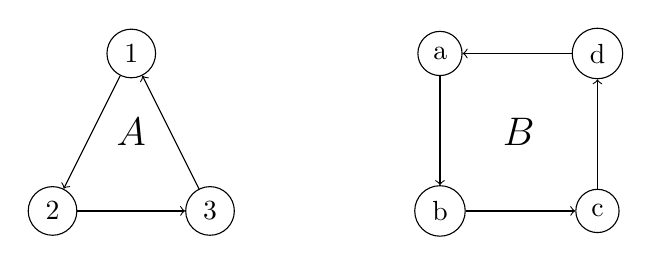
\begin{tikzpicture}[every node/.style={draw,circle}, baseline=(current bounding box.north)]
    \begin{scope}[xshift=-70]
    \node[draw=none, font=\Large] {$\str{A}$};
    \path[->]
      (0,1) node(n1) {1}
      (-1,-1) node(n2) {2}
      (1,-1) node(n3) {3}
      (n1) edge (n2)
      (n2) edge (n3)
      (n3) edge (n1);
    \end{scope}

    \node[draw=none, font=\Large] {$\bisimto_{\GF}$};

    \begin{scope}[xshift=70]
    \node[draw=none, font=\Large] {$\str{B}$};
    \path[->]
      (-1,1) node(n1) {a}
      (-1,-1) node(n2) {b}
      (1,-1) node(n3) {c}
      (1,1) node(n4) {d}
      (n1) edge (n2)
      (n2) edge (n3)
      (n3) edge (n4)
      (n4) edge (n1);
    \end{scope}
  \end{tikzpicture}
  \end{figure}
  By design we clearly have $\str{A}\models \varphi$ and $\str{B} \not\models \varphi$. On the other hand, $\str{A}$ and $\str{B}$ are $\GF$-bisimilar, witnessed by the bisimulation $\bisimZ$ consisting of the partial isomorphisms:
  \begin{itemize}
    \item $s_{1} \mapsto t_{1}$ for every $s_{1} \in \{1,2,3\}$ and $t_{1} \in \{a,b,c,d\}$, and
    \item $s_{1}s_{2} \mapsto t_{1}t_{2}$ for every $s_{1}s_{2} \in \{12,23,31\}$ and $t_{1}t_{2} \in \{ab,bc,cd,da\}$
  \end{itemize}
  where $s_{1}s_{2} \mapsto t_{1}t_{2}$ denotes the partial isomorphism mapping the element $s_{1}$ to $t_{1}$ and the element $s_{2}$ to $t_{2}$.
\end{example}

\noindent
Now a similar characterisation can be provided for $\FGF$. 
Due to the ``forwardness'' of the underlying logic, it is convenient to think about maps as tuples.
A \emph{system of forward partial maps} between structures $\str{A}$ and $\str{B}$ is any non-empty subset of $\bigcup_{i=1}^{\infty} (A^i \times B^i)$ satisfying:
\begin{description}\itemsep0em
  \item[\desclabel{(AtomicEq)}{bisim:atomiceq}] For all $(\elemtuplea, \elemtupleb) \in \bisimZ$ we have that $\elemtuplea$, $\elemtupleb$ are live and $\atp{\FGF}{\str{A}}{\elemtuplea} = \atp{\FGF}{\str{B}}{\elemtupleb}$~holds.
\end{description}
For our fixed signature $\Sigma$, the infinite union $\bigcup_{i=1}^{\infty} (A^i \times B^i)$ in this definition may be replaced by the finite union $\bigcup_{i=1}^{\arity(\Sigma)} (A^i \times B^i)$, since live tuples cannot have more than $\arity(\Sigma)$ components.
If $\bisimZ, \bisimZ'$ are systems of forward partial maps between $\str{A}$ and $\str{B}$, we say that $\bisimZ'$ satisfies back-and-forth conditions for $\bisimZ$ if for every $(\elemtuplea, \elemtupleb) \in \bisimZ$ the following conditions hold:
\begin{description}\itemsep0em
  \item[\desclabel{(fForth)}{bisim:fforth}] For every (possibly empty) infix $\elemtuplecfromto{i}{j}$ of $\elemtuplec$ and a live tuple $\elemtuplee$ in $\str{A}$ such that $\elemtuplecfromto{i}{j} = \elemtupleefromto{1}{j{-}i{+}1}$ there is a live tuple $\elemtuplef$ with $\elemtupledfromto{i}{j} = \elemtupleffromto{1}{j{-}i{+}1}$ such that $(\elemtuplee, \elemtuplef) \in \bisimZ'$ holds.
  %
  \item[\desclabel{(fBack)}{bisim:fback}] For every (possibly empty) infix $\elemtupledfromto{i}{j}$ of $\elemtupled$ and a live tuple $\elemtuplef$ in $\str{B}$ such that $\elemtupledfromto{i}{j} = \elemtupleffromto{1}{j{-}i{+}1}$ there is a live tuple $\elemtuplee$ with $\elemtuplecfromto{i}{j} = \elemtupleefromto{1}{j{-}i{+}1}$ such that $(\elemtuplee, \elemtuplef) \in \bisimZ'$~holds.
\end{description}
A system of forward partial maps $\bisimZ$ between $\str{A}$ and $\str{B}$ is an $\FGF$-\emph{bisimulation} between $\str{A}$ and $\str{B}$ if it itself satisfies the above conditions.
An $\ell$-$\FGF$-bisimulation between $\str{A}$ and $\str{B}$ is a sequence $\bisimZ_0, \bisimZ_1, \ldots, \bisimZ_\ell$ of systems of forward partial maps between $\str{A}$ and $\str{B}$ such that for all $i < \ell$ we have that $\bisimZ_i$ satisfies~\ref{bisim:fforth} and~\ref{bisim:fback} conditions for $\bisimZ_{i{+}1}$.
We~speak about $\FGF$-\emph{bisimilar} and $\ell$-$\FGF$-\emph{bisimilar} (pointed) structures in total analogy to the guarded-fragment case.
We stress that the back-and-forth conditions allow for choosing an empty infix, so $\ell$-$\FGF$-bisimulations are not limited to the local neighbourhood of some tuple.
Instead, even for $\ell = 1$, every guarded tuple must be mapped to a tuple in the other structure.

A ``forward'' counterpart of \cref{lemma:GF-bisimulations-work-well} is presented below.
\begin{lemma}\label{lem:FGF-bisimulations-work-well}
For every pair of pointed structures $(\str{A}, \elemtuplea)$ and~$(\str{B}, \elemtupleb)$ we have that:
\begin{enumerate}[(a)]
\item $(\str{A}, \elemtuplea) \bisimto_{\FGF} (\str{B}, \elemtupleb)$ implies $(\str{A}, \elemtuplea) \equiv_{\FGF} (\str{B}, \elemtupleb)$;
\item $(\str{A}, \elemtuplea) \bisimto_{\FGF}^{\ell} (\str{B}, \elemtupleb)$ implies $(\str{A}, \elemtuplea) \equiv_{\FGF_\ell} (\str{B}, \elemtupleb)$ for all $\ell \in \N$;
\end{enumerate}
Moreover, the converse holds for $\omega$-saturated $\str{A}$ and $\str{B}$.
\end{lemma}
\begin{proofsketch}
  A proof for condition \textbf{(a)} is provided in~\cite[Lemma 3]{BednarczykJ22}.
  The proof for condition \textbf{(b)} uses the same ideas as the proof for \textbf{(a)}.
  \begin{itemize}
    \item
          For the ``if'' direction, we perform induction over $\ell$ and use~\ref{bisim:fforth} to obtain a witness in $\str{B}$ for every existential quantifier that has a witness in $\str{A}$ (by properties of $\models$, it suffixes to consider existential quantifiers as $\forall\vartuplex\ \cdots \iff \lnot \exists \vartuplex\ \cdots$).
    \item
          For the opposite direction, we show that the set of pairs of tuples from $\str{A}$ and $\str{B}$ with the same $\FGF_{\ell}$-type is an $\ell$-$\FGF$-bisimulation.
          Let $\elemtuplec \sqin A$ and $\elemtupled \sqin B$ be live tuples with equal $\FGF_{\ell}$-types.
          Consider any tuple $\elemtuplee$ extending an infix $\elemtuplecfromto{i}{j}$ to a new live tuple $\elemtuplecfromto{i}{j}\elemtuplee$.
          Let $\Gamma$ be the $\FGF_{k-1}$-type of $\elemtuplee$ with regards to $\elemtuplecfromto{i}{j}$.
          Because of $\omega$-saturation, this type is realized in $\str{B}$ if every of its finite subsets is realized.
          For every finite subset of $\Gamma$, we can construct an $\FGF_{k}$-formula that asserts the existence of a witness realizing this finite $\FGF_{k-1}$-type.
          Hence by $k$-$\FGF$-equivalence, there exists a tuple $\elemtuplef$ that extends $\elemtupledfromto{i}{j}$ and same $\FGF_{k-1}$-type.
          Therefore, the set of pairs of tuples with equal $\FGF_{\ell}$-types is an $\ell$-$\FGF$-bisimulation, satisfying the theorem.
  \end{itemize}
\end{proofsketch}
%!TEX root = ../main.tex

\begin{proof}
  A proof for condition \textbf{(a)} is provided in~\cite[Lemma 3]{BednarczykJ22}, and thus we proceed with condition \textbf{(b)}.
  We start from the ``if'' direction. 
  Let us fix $\sigma$-structures $\str{A}$ and $\str{B}$.
  We want to establish that for all $\ell \in \N$, $\elemtuplea$ in $\str{A}$, and $\elemtupleb$ in $\str{B}$ the following condition holds:
  \[
    (\heartsuit_\ell)(\elemtuplea, \elemtupleb){:} \ \ \ \  (\str{A}, \elemtuplea) \bisimto_{\FGF[\sigma]}^{\ell} (\str{B}, \elemtupleb) \ \text{implies} \ (\str{A}, \elemtuplea) \equiv_{\FGF_\ell[\sigma]} (\str{B}, \elemtupleb).
  \]
  We proceed by induction. 
  For the inductive base, take any $\elemtuplea$ from $\str{A}$, any $\elemtupleb$ from $\str{B}$, and suppose that the antecedent of $(\heartsuit_0)(\elemtuplea,\elemtupleb)$ holds.
  Thus, by \ref{bisim:atomiceq} we know that $\elemtuplea$ and~$\elemtupleb$ have equal $\FGF[\sigma]$-types.
  This means that for all atomic $\varphi$ of $\FGF[\sigma]$ we have $\str{A} \models \varphi[\elemtuplea]$ if and only if $\str{B} \models \varphi[\elemtupleb]$.
  Hence, by a routine case analysis employing obvious properties of $\models$ relation, the above equivalence is lifted to the case of all quantifier-free $\FGF[\sigma]$-formulae, establishing the consequent of $(\heartsuit_0)(\elemtuplea,\elemtupleb)$.
  For the inductive step, fix any positive $\ell$ and assume that for all $k$ smaller than $\ell$ and the condition $(\heartsuit_k)(\elemtuplea,\elemtupleb)$ is satisfied for all tuples $\elemtuplea$ and $\elemtupleb$.
  Now take any tuple $\elemtuplea$ from $\str{A}$ and $\elemtupleb$ from $\str{B}$.
  To show the consequent of $(\heartsuit_\ell)(\elemtuplea,\elemtupleb)$, we take any formula $\varphi(x_1, \ldots, x_n) \in \FGF_\ell[\sigma]$.
  If the quantifier rank of $\varphi$ is smaller than $\ell$, then we are done by $(\heartsuit_{\ell{-}1})(\elemtuplea,\elemtupleb)$.
  Hence, suppose that the quantifier rank of $\varphi$ is precisely~$\ell$.
  By structural induction (relying on properties of $\models$ relation) it amounts to establish the equivalence for $\varphi$ in one of the following forms: 
  \begin{itemize}\itemsep0em

  \item $\varphi$ is of the form $\exists{\vartuplexfromto{n{+}1}{m}}\ \relR(\vartuplexfromto{i}{j}) \land \psi(\vartuplexfromto{i}{j})$, where a predicate $\relR$ serves as a guard, $i \geq 1$ and $j \leq m$.
  Note that the quantifier rank of $\relR(\vartuplexfromto{i}{j}) \land \psi(\vartuplexfromto{i}{j})$ is less than $\ell$.
  Suppose that $\str{A} \models \varphi[\elemtuplea]$ (the case of $\str{B} \models \varphi[\elemtupleb]$ is symmetric).
  Let $\elemtuplec$ be the (possibly empty) infix $\elemtupleafromto{i}{n}$ of~$\elemtuplea$.
  Then there exists a (possibly empty) tuple $\elemtuplee$ in $\str{A}$ such that $\str{A} \models \relR[\elemtuplec\elemtuplee] \land \psi[\elemtuplec\elemtuplee]$.
  Note that $\elemtuplec\elemtuplee$ is $\sigma$-live. 
  By~\ref{bisim:fforth}\bfside{This requires that $\elemtuplea$ is live. Is this true? Example: $\varphi = \relS(x_{1}, x_{2}) \land \relT(x_{3}) \land \exists{x_{4}} (\relH(x_{2}, x_{3}, x_{4}))$ (according to our definitions, this should be an FGF-formula with free variables $x_{1}, x_{2}, x_{3}$, right?) could be satisfied at an $\elemtuplea$ that is not guarded. Perhaps we want to require that the free variables of formulae are guarded as well?} we can find a (possibly empty) tuple $\elemtuplef$ in $\str{B}$ such that $(\str{A}, \elemtuplec\elemtuplee) \bisimto_{\FGF[\sigma]}^{\ell{-}1} (\str{B}, \elemtupled\elemtuplef)$ for~$\elemtupled$ equal to $\elemtuplebfromto{i}{n}$.
  Applying inductive hypothesis, namely $(\heartsuit_{\ell{-}1})(\elemtuplec\elemtuplee,\elemtupled\elemtuplef)$, we know that the consequent of $(\heartsuit_{\ell{-}1})(\elemtuplec\elemtuplee,\elemtupled\elemtuplef)$ holds true.
  This clearly implies $\str{B} \models \relR[\elemtupled\elemtuplef] \land \psi[\elemtupled\elemtuplef]$, which finally lead us to $\str{B} \models \varphi[\elemtupleb]$.

  \item $\varphi$ is of the form $\exists{x_{1}} \psi(x_1)$. Then the quantifier rank of $\psi$ is less than $\ell$.
  Suppose that $\str{A} \models \varphi[\elemtuplea]$ (the case of $\str{B} \models \varphi[\elemtupleb]$ is symmetric).
  Then there exists an element $\elem{c}$ in $\str{A}$ for which $\str{A} \models \psi[\elem{c}]$.
  As $\elem{c}$ is trivially guarded, we apply~\ref{bisim:fforth} to find $\elem{d}$ in $\str{B}$ for which $(\str{A}, \elem{c}) \bisimto_{\FGF[\sigma]}^{\ell{-}1} (\str{B}, \elem{d})$.
  Note that $\ell{-}1$ is non-negative by positivity of $\ell$. 
  Thus, by $(\heartsuit_{\ell{-}1})(\elem{c},\elem{d})$ we know that $(\str{A}, \elem{c}) \equiv_{\FGF_{\ell{-}1}[\sigma]} (\str{B}, \elem{d})$ holds. 
  In particular, this implies $\str{B} \models \psi[\elem{d}]$, concluding the proof.
\end{itemize}

For the opposite direction, take $\ell \in \N$ and a pair of $\omega$-saturated pointed $\sigma$-structures $(\str{A}, \elemtuplea)$ and $(\str{B}, \elemtupleb)$.
Suppose that $(\str{A}, \elemtuplea) \equiv_{\FGF_\ell[\sigma]} (\str{B}, \elemtupleb)$.
We construct a family $\bisimZ_0, \ldots, \bisimZ_\ell$ of systems of forward partial maps as follows:
\[
  \bisimZ_\mathit{k} \coloneqq \{ (\elemtuplec, \elemtupled) \in \bigcup_{i=0}^{\infty} (A^i \times B^i) \mid  (\str{A}, \elemtuplec) \equiv_{\FGF_\mathit{k}[\sigma]} (\str{B}, \elemtupled), \ \text{and} \ \elemtuplec, \elemtupled \ \text{are $\sigma$-live} \}. 
\]
We claim that such a family is an $\ell$-$\FGF[\sigma]$-bisimulation between $(\str{A}, \elemtuplea)$ and $(\str{B}, \elemtupleb)$. 
Note that the condition \ref{bisim:atomiceq} is trivially satisfied by all the $\bisimZ_\mathit{k}$ above, and that $(\elemtuplea, \elemtupleb)$ belongs to all the sets $\bisimZ_\mathit{k}$ by design.
Thus it suffices to show that for all $\mathit{k} \in \{ 1, 2, \ldots, \ell\}$ that the system of forward partial
maps $\bisimZ_\mathit{k}$ satisfies \ref{bisim:fforth} and \ref{bisim:fback} for $\bisimZ_{\mathit{k}{-}1}$.
Hence, take any such $j$ and let us proceed with a proof of \ref{bisim:fforth} (the case of \ref{bisim:fback} is symmetric). 
Let $(\elemtuplec, \elemtupled) \in \bisimZ_\mathit{k}$, $\elemtuplecfromto{i}{j}$ be a (possibly empty) infix of $\elemtuplec$
and $\elemtuplee$ be any tuple in $\str{A}$ such that $\elemtuplecfromto{i}{j}\elemtuplee$ is $\sigma$-live.
We are going to show that the set 
\[
  \Gamma \deff \{ \varphi \mid \str{A} \models \varphi[\elemtuplecfromto{i}{j}\elemtuplee], \varphi \in \FGF_{\mathit{k}{-}1}[\sigma] \}
\] 
is realized in $\str{B}$ by $\elemtupledfromto{i}{j}\elemtuplef$ for some $|\elemtuplee|$-tuple $\elemtuplef$ from $\str{B}$.
By $\omega$-saturation of $\str{B}$ it suffices
to establish that any finite subset of $\Gamma$ is realized by $\elemtupledfromto{i}{j}\elemtupleh$ for some $|\elemtuplee|$-tuple $\elemtupleh$. 
Let $\Delta$ be a finite subset of $\Gamma$.
By design, we have 
$(\str{A}, \elemtuplecfromto{i}{j}) \models \exists{\vartuplex} \textstyle\bigwedge \Delta$.\bbeside{Change $\bar{x}$... Btw, why is this in $\FGF$? Explain. use the guard of $\bar{c}\bar{e}$.}
Moreover, as $\exists{\vartuplex} \textstyle\bigwedge \Delta$ is an $\FGF_\mathit{k}$-formula,
we can invoke $\mathit{k}$-$\FGF$-equivalence of $(\str{A}, \elemtuplec)$ and $(\str{B}, \elemtupled)$ to deduce~$(\str{B}, \elemtupledfromto{i}{j}) \models \exists{\vartuplex} \textstyle\bigwedge \Delta$.
This implies that $\Gamma$ is indeed realized in $\str{B}$, and let $\elemtupledfromto{i}{j}\elemtuplef$ be a tuple witnessing this fact.
By the choice of $\Gamma$, we know that  $(\str{A}, \elemtuplecfromto{i}{j}\elemtuplee) \equiv_{\FGF_{\mathit{k}{-}1}[\sigma]} (\str{B}, \elemtupledfromto{i}{j}\elemtuplef)$, and hence
$(\elemtuplecfromto{i}{j}\elemtuplee, \elemtupledfromto{i}{j}\elemtuplef) \in \bisimZ_{\mathit{k}{-}1}$. 
This concludes the proof of that $\bisimZ_{\mathit{k}}$ satisfies \ref{bisim:fforth}, and thus concludes the proof that the family $\bisimZ_0, \ldots, \bisimZ_\ell$ is an $\ell$-$\FGF[\sigma]$-bisimulation between $(\str{A}, \elemtuplea)$ and $(\str{B}, \elemtupleb)$. 
\end{proof}


The following example presents two structures that are $\FGF$-bisimilar but not $\GF$-bisimilar.
\begin{example}
  Consider the two structures $\str{A} := \tikz[baseline=-0.5ex]{\path[->] (0,0) node[draw,circle] (n1) {} (n1) edge[loop above,in=70,out=110,looseness=10] (n1);}$ and $\str{B} := \tikz[baseline=-0.5ex]{\path[->] (0,0) node (n1) [draw,circle] {} (3em,0) node (n2) [draw,circle] {} (n1) edge[bend left] (n2) (n2) edge[bend left] (n1);}$ with a binary predicate $\relE$ interpreted as edges. These two structures are $\FGF[\{\relE\}]$-bisimilar, while a $\GF$-sentence $\exists{\varx_1}\relE(\varx_1,\varx_1)$ can distinguish them.

\end{example}

Both $\GF$-bisimulation and $\FGF$-bisimulation naturally correspond to games~\cite[Sec. 1.2.1]{Gradel014}.
We focus on the the game corresponding to $\FGF$-bisimulation here.
The $\FGF$-\emph{bisimulation game} is played on two pointed structures $(\str{A}, \elemtuplea)$ and $(\str{B}, \elemtupleb)$ by two players, Spoiler and Duplicator.
The game starts by selecting the tuples $\elemtuplea$ and $\elemtupleb$ from the corresponding structures.
Throughout the game, Duplicator must maintain the condition that the two currently selected tuples have equal atomic-$\FGF$-types.
If $\elemtuplea$ and $\elemtupleb$ already do not have the same atomic $\FGF$-type, then Duplicator loses instantly.
Otherwise, the game proceeds in rounds.
In each round, Spoiler first chooses a structure.
As the game is symmetric, let us assume that spoiler chooses the structure $\str{A}$.
Spoiler then selects an infix $\elemtupleafromto{i}{j}$ of the currently selected tuple and a new live tuple $\elemtuplec$ which has $\elemtupleafromto{i}{j}$ as a prefix.
For convenience, we use the terms \emph{shared elements} for the prefix $\elemtuplecfromto{1}{j-i+1}$ and \emph{unshared elements} for the remaining elements, namely $\elemtuplecfromto{j-i+1+1}{|\elemtuplec|}$.
Duplicator, in order to continue the game, must then find a live tuple $\elemtupled$ in $\str{B}$ having $\elemtuplebfromto{i}{j}$ as prefix such that $\elemtuplec$ and $\elemtupled$ have equal $\FGF$-types.
Note that Spoiler may choose an index $j$ that is not maximal, so that the situation of $a_{j+1} = c_{j-i+1+1}$ is still possible.
We still regard $c_{j-i+1+1}$ as an unshared element, since Duplicator is allowed to pick a tuple $\elemtupled$ where $b_{j+1} \neq d_{j-i+1+1}$.
The game then continues with the next round, with $\elemtuplec$ and $\elemtupled$ as the new starting tuples.
Spoiler wins the game if Duplicator is unable to respond, i.e.\ to find suitable tuples.
Duplicator wins otherwise.
It is easy to see that the possible moves of Spoiler are analogous to the back-and-forth conditions for $\FGF$-bisimulation, as is also the case for the $\GF$-game~\cite[Sec.\ 3.2]{Gradel014}.
To win, Duplicator must be able to respond to any move that Spoiler makes.
A winning strategy for Duplicator thus corresponds to an $\FGF$-bisimulation between the two structures, and vice-versa.
If we restrict the game to only $\ell$-rounds, where the winning condition for Duplicator is that Spoiler cannot win in the first $\ell$-rounds, then the game is equivalent (in the aforementioned sense) to the existence of an $\ell$-FGF-bisimulation between $\str{A}, \elemtuplea$ and $\str{B}, \elemtupleb$.
We collect these observations in the following corollary:

\begin{corollary}
  In the $\FGF$-game played on structures $\str{A}, \elemtuplea$ and $\str{B}, \elemtupleb$:
  \begin{itemize}
    \item Duplicator has as winning strategy if and only if $\str{A}, \elemtuplea \bisimto_{\FGF} \str{B}, \elemtupleb$,
    \item Duplicator has a winning strategy for $\ell$ rounds if and only if $\str{A}, \elemtuplea \bisimto_{\FGF}^{\ell} \str{B}, \elemtupleb$.
  \end{itemize}
\end{corollary}
